\chapter{Technologien für Multi-Wan Bonding}
\label{chap:verwendeteTechnologien}
\section{Multi-Wan Bonding}
Multi-Wan Bonding beschreibt, wie der Name schon sagt, das Bündeln einer Verbindung über mehrere WAN Zugänge. Im Normalfall handelt es sich bei WAN um das Internet. 
\\\\
Es werden dabei verschiedene WAN-Anbindungen wie LTE, Kabel, Glasfaser, vDSL, DSL und Satellit miteinander gekoppelt, um eine ausfallsichere und schnellere Verbindung zu erhalten. Die Bandbreiten der einzelnen WAN-Anbindungen wird dabei fast summiert. 

\subsection{Einsatzgebiete}
Multi-Wan Bonding kommt vorallem dann zum Einsatz, wenn eine besonders stabile Verbindung benötigt wird. Auch das Erhöhen der Bandbreite ist ein möglicher Einsatzzweck, hierfür gibt es aber bessere Lösungen.
\\\\
Hauptsächlich wird Multi-Wan Bonding in Unternehmensnetzwerken verwendet, die eine besonders hohe Erreichbarkeit/Stabilität benötigen. Oft ist es aber nicht möglich, überall eine stabile Verbindung zu erreichen. Befindet sich eine Produktionsstätte an einem abgelegenen Ort mit schlechter Infrastruktur, so ist die Gefahr einer instabilen Verbindung sehr groß. Da immer die sekundenaktuellen Informationen benötigt werden, würde dies zu einem Produktionsstop führen. Multi-Wan Bonding kann eine mögliche Lösung sein, um die Produktionsstätte hochverfügbar zu machen.
\\\\
Auch für Video/Audio-Streaming von Unterwegs eignet sich Multi-Wan Bonding sehr. So kann beispielsweise ein Twitch Streamer von Unterwegs mehrere SIM-Karten unterschiedlicher LTE Netzbetreiber zeitgleich verwenden, um so sicherzustellen, dass sein Stream, selbst wenn eines der Netze nicht mehr erreichbar ist nicht, unterbrochen wird.

\newpage
\subsection{Unterschied zu einer Normalen Verbindung}
\begin{figure}[h]
    \centering
    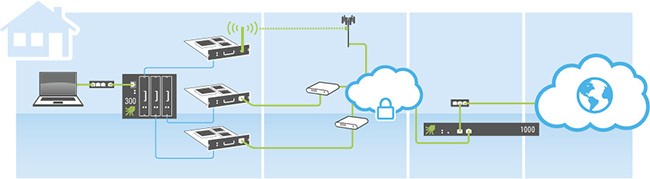
\includegraphics[width=1\textwidth]{WANB.jpg}
    \caption[Multi-WAN Bonding Konzept]{Multi-WAN Bonding Konzept}[\cite{WANB}]
\end{figure}
\noindent
Im Vergleich zu einer Normalen Verbindungsmethode handelt es sich beim Multi-Wan Bonding um eine Art von VPN Tunnel. Datenpakete laufen nicht wie gewöhnlich direkt über eine Leitung sondern werden beim Betreten des VPN Tunnels von einer Software oder Hardware Multi-Wan Lösung auf mehrere Leitungen aufgeteilt. Dies alleine ist jedoch noch nicht ganz ausreichend. Um wieder eine Verbindung zu bekommen die sich auch verwenden lässt, ist es notwendig, diese aufgeteilten Datenpakete wieder zusammen zu führen. Es gibt also einen entfernten Endpunkt, der als Proxy fungiert. Dieser Endpunkt empfängt die Datenpakete, die über die verschiedenen Verbindungen hinausgesandt wurden und setzt diese wieder zu einem Datenstrom zusammen. Damit stellt er das Ende des VPN Tunnels dar. 
\\\\
Es kommt dadurch selbstverständlich zu einem kleinen Datenüberhang im vergleich zu einer direkten Verbindung, da Metadaten zur Steuerung des VPN Tunnels benötigt werden. Oft werden übertragene Daten im Tunnel auch verschlüsselt.
\\\\
Da die Daten, wie bereits erwähnt, über verschiedene Verbindungen übertragen werden, die sich auch in ihrer Stabilität, Geschwindigkeit und Übertragungszeit stark unterscheiden können, muss laufend darauf geachtet werden den Datenstrom entsprechend den aktuellen Leistungs charakteristika der einzelnen Tunnel Datenströme aufzuteilen. Dies geschieht vollkommen automatisch durch die verwendete Multi-Wan Bonding Lösung und erfordert kein manuelles Eingreifen durch den Anwender.

\subsection{Unterschied zu Load Balancing}
Auch beim Load Balancing werden, wie beim Multi-Wan Bonding, mehrere WAN Verbindungen verwendet. Die auch im gleichen Maße vielfältig sein können.
\\\\
Der entscheidende Unterschied zum Multi-Wan Bonding besteht darin, dass hier das Aufteilen auf Session-Ebene stattfindet. Hier werden Sessions über den WAN Zugang laufen gelassen, der gerade am meisten Ressourcen frei hat. Beim Wan Bonding hingegen wird auf Datenpaket-Ebene aufgeteilt. Das Aufteilen auf Session-Ebene bringt Vor und Nachteile die im Folgenden dargestellt werden.
\newpage
\paragraph{Load-Balancing Vorteile:}
\begin{enumerate}
    \item Es wird kein entfernter Endpunkt benötigt.
    \item Es gibt keinen Datenüberhang bei der Verbindung.
    \item Aufgrund eines verringerten Verarbeitungsaufwandes ist der Ping besser. 
\end{enumerate}
\paragraph{Load-Balancing Nachteile:}
\begin{enumerate}
    \item Bandbreite wird nicht gebündelt.
    \item Fällt eine der WAN Verbindungen aus, werden auch alle Sessions, die über diese Verbindung laufen, unterbrochen.
    \item Die Stabilität ist schlechter.
    \item Sessions haben verschiedene IP-Adressen je nach verwendeter WAN Verbindung.
\end{enumerate}


\section{IP Routing Table}
Der IP Routing Table oder Routing Table ist eine Tabelle, die alle Hosts, die an einem Netzwerk angeschlossen sind, aufbauen. Diese Tabelle wird von dem Betriebssystem verwendet um IP Pakete weiter- oder umzuleiten. Durch diese Informationen ist es außerdem möglich die Topologie des Netzwerkes, in dem sich der Host befindet, zu bestimmen.\footnote[1]{\cite[Vgl.][]{2}}
\\\\
Einträge in das Routing Table können entweder manuell, in Form von statischen Routen oder dynamisch, über Routing Protokolle erstellt werden.$^{1}$
\\\\
Ein Eintrag des Routing Table unter Linux und unter Windows hat folgende 5 Attribute: ein Netzwerkziel, eine Netzwerkmaske, ein Gateway, eine Schnittstelle und eine Metrik.$^{1}$
\\\\
Das Netzwerkziel und die Netzwerkmaske zusammen beschreiben, an welches Netzwerk ein IP Paket gerichtet sein muss, um von diesem Eintrag beeinflusst zu werden. Hier gibt es jedoch eine besondere Einstellung, wenn das Netzwerkziel als auch die Netzwerkmaske nur aus Nullen besteht. Diese Einträge werden als default Routen bezeichnet. Default Routen beeinflussen alle Pakete, bei denen folgendes \textbf{nicht} zutrifft$^{1}$: 
\\
\begin{itemize}
    \item Es gibt keinen anderen default Routen mit einer niedrigeren Metrik.
    \item Pakete wurden vorher noch nicht von einem spezifischeren Eintrag umgeleitet.
\end{itemize}
\ \\
Das Gateway beschreibt den nächsten Hop. Genauer gesagt spiegelt es die IP-Adresse des Hosts wieder, um welches das IP-Paket umgeleitet werden muss, um in das Zielnetzwerk, oder in ein Netzwerk, das mit dem Zielnetzwerk verbunden ist, zu gelangen.$^{1}$
\\\\
Die Metrik gibt an, welcher Eintrag verwendet werden soll, wenn mehrere Einträge gleiche Werte im Netzwerkziel und in der Netzwerkmaske haben. Sie gibt bei dynamischen Routen an, wie viele Hops das IP Paket braucht, um beim Gateway anzukommen. Deswegen wird auch die kleinere Metrik bevorzugt, weil weniger Hops in der Regel weniger Latenz bedeuteten.$^{1}$
\newpage
\noindent
Die Schnittstelle gibt an, über welche Network Interface Card (NIC) das IP Paket geleitet werden muss, damit es das Gateway erreichen kann.\footnote[1]{\cite[Vgl.][]{2}}
\\\\
Eine Routing Tabelle kann wie folgt aussehen:
\\
\begin{center}
    \begin{tabular}{| c | c | c | c | c |}
        \hline
        Netzwerkziel & Netzwerkmaske & Gateway & Schnittstelle & Metrik \\
        \hline
        0.0.0.0 & 0.0.0.0 & 172.168.0.10 & 172.168.0.1 & 30 \\
        172.163.241.22 & 255.255.255.255 & 10.0.0.2 & 10.0.0.1 & 22 \\
        \hline
    \end{tabular}
\end{center}
\ \\
Bei diesem Beispiel wird ein Paket mit der IP-Adresse 172.163.241.22 an die IP-Adresse 10.0.0.2 über die Schnittstelle 10.0.0.1 weitergeleitet. Ein Paket mit IP-Adresse 30.20.10.0 wird an die IP-Adresse 172.168.0.10 über die Schnittstelle 172.168.0.1 weitergeleitet.


\section{Network Address Translation (NAT)}
NAT (Network Address Translation) dient zur Verbindung zweier getrennter Netzwerke. Im häufigsten Fall zwischen dem Internet und einem lokalen Netzwerk. Der größte Unterschied zum normalen Routing ist dabei, dass das lokale Netzwerk mit seinen IP-Adressen im Internet bzw. dem außerhalb liegenden Netzwerk nicht registriert ist. Dies hat natürlich auch zur Folge, dass IP-Adressen im lokalen Netzwerk nicht vom äußeren Netzwerk aus erreichbar sind. 
\subsection{Wie funktioniert NAT?}
Wie der Name Network Address Translation (= Netzwerkadressübersetzung) schon sagt, werden dabei die nicht unbedingt global eindeutigen IP-Adressen des internen Netzwerks auf eine oder mehrere Adressen im größeren Netzwerk übersetzt. Dies geschieht gewöhnlich durch ein einzelnes Gerät z.b. einem Router. Dieser Router besitzt sowohl im lokalen unregistriertem Netzwerk eine IP-Adresse als auch im größeren Netzwerk.
\\\\
Erreicht den Router nun ein Datenpaket vom lokalen Netzwerk, das für eine IP-Adresse bestimmt ist, die nicht im lokalen Netzwerk liegt, so leitet er dieses Paket in das äußere Netzwerk weiter. Da die IP-Adressen vom lokalen Netzwerk im äußerem Netzwerk jedoch nicht bekannt sind, hätte nun der Empfänger im äußerem Netzwerk keine Möglichkeit zu antworten. Um dieses Problem zu lösen, kommt nun der eigentliche NAT-Vorgang zum tragen. 


\newpage
\begin{figure}[h]
    \centering
    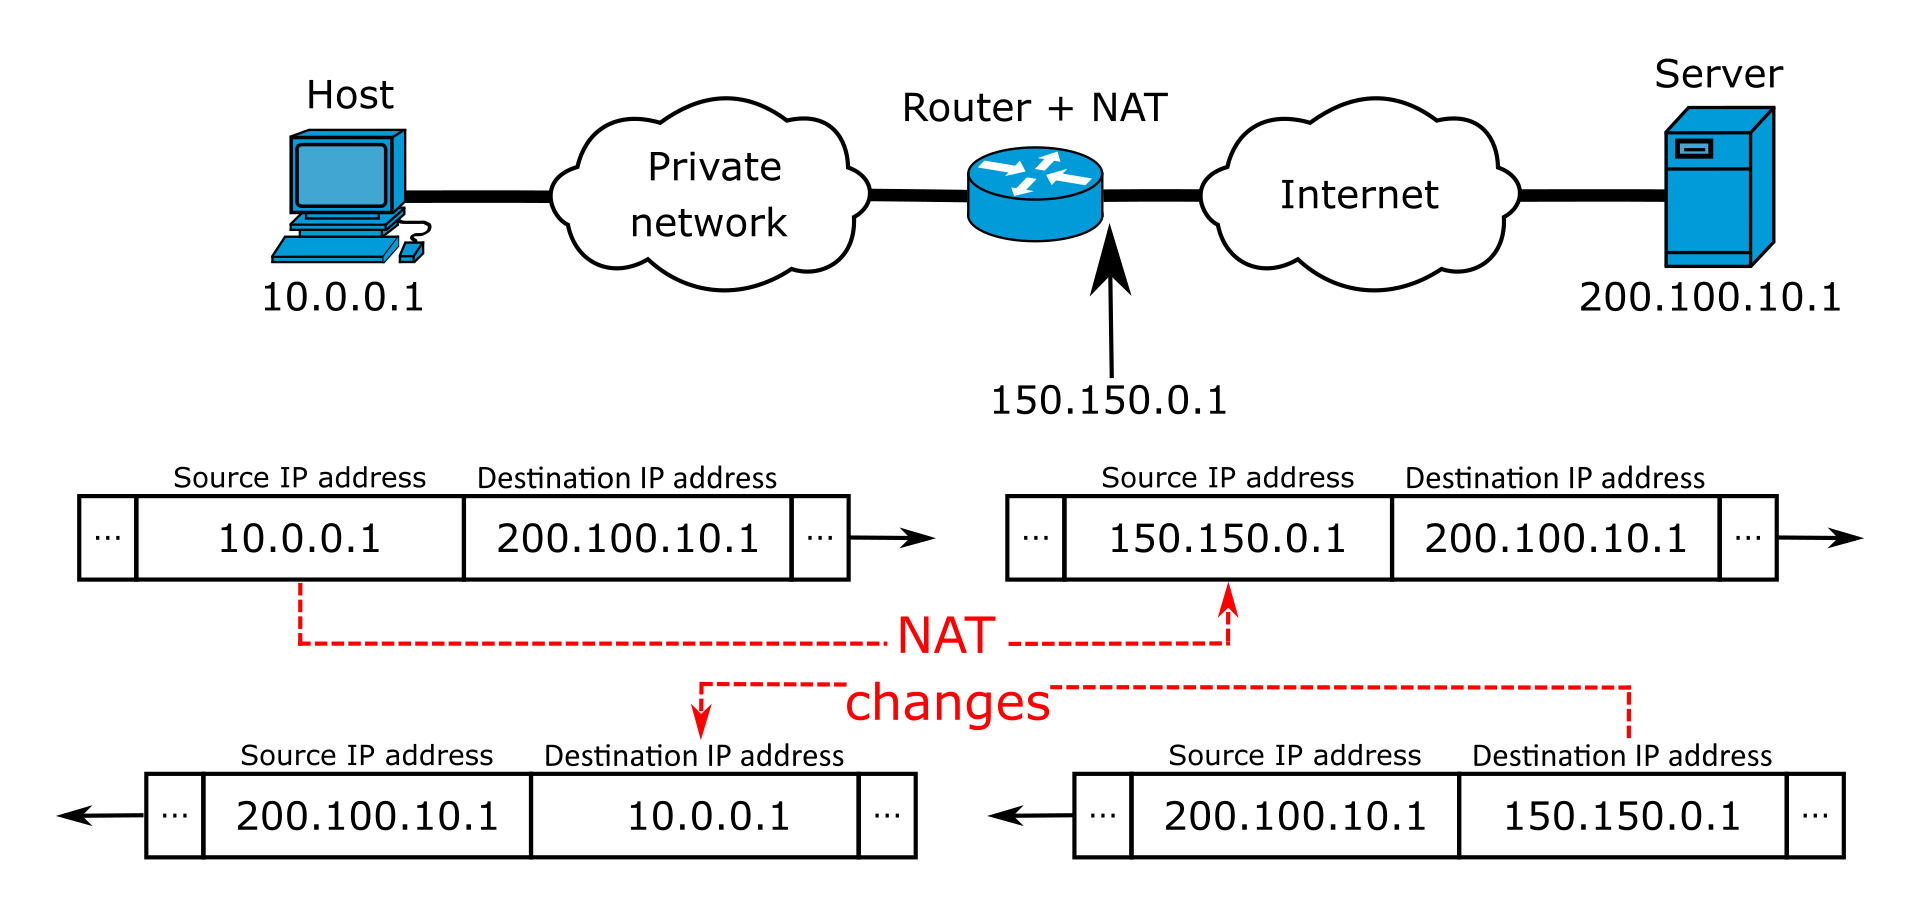
\includegraphics[width=1\textwidth]{NAT1.png}
    \caption[NAT Konzept]{NAT Konzept}[\cite{NATi1}]
\end{figure}
\noindent
Der Router der, als Mittelsmann zwischen den Netzwerken agiert, tauscht die Absenderadresse im IP-Header des lokalen Packets gegen seine eigene im äußeren Netzwerk registrierte IP-Adresse aus. Dadurch ist es nun einem Host im äußeren Netzwerk möglich, auf das Datenpaket zu antworten. 
\\\\
Kommt nun eine Antwort wieder beim Router an, wird die Ziel IP-Adresse gegen die des ursprünglichen Anfragestellers aus dem lokalen Netzwerk ausgetauscht, um im lokalen Netzwerk zugestellt werden zu können.

\newpage
\subsection{NAT Übersetzungs Tabelle}
Woher weiß nun der Router für welchen Host im lokalen Netzwerk die Antwort aus dem äußeren Netzwerk bestimmt war? 
\begin{figure}[h]
    \centering
    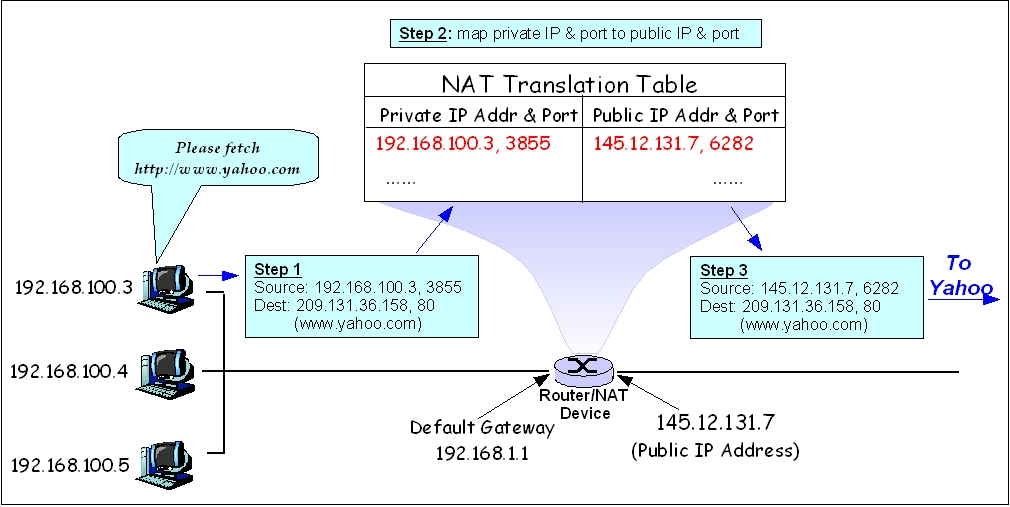
\includegraphics[width=1\textwidth]{NAT2.jpg}
    \caption[NAT Übersetzungs Tabelle]{NAT Übersetzungs Tabelle}[\cite{NATi2}]
\end{figure}
Beim Absenden der Anfrage durch den lokalen Host merkt sich der Router in der sogenannten NAT Tabelle den ursprünglichen Port und die lokale IP-Adresse, bevor er im NAT Prozess diese durch einen eigenen gewählten Port und eine eigene registrierte IP-Adresse im größerem Netz ersetzt, die er ebenfalls in die Tabelle einträgt. 
Kommt nun eine Antwort auf genau diesen äußeren Endpunkt (äußere IP-Adresse und gewählter Port vom NAT Prozess), so holt sich der Router aus der NAT Tabelle einfach die ursprüngliche Absenderadresse und den Port und setzt diese im empfangenen Antwortpaket als Zieladresse und Zielport ein. 
\subsection{NAT und OSI Schichten}
Da der NAT Vorgang auch einen Port benötigt, ist ersichtlich, das NAT auf OSI Schicht “4 Transport” arbeitet. Das ist natürlich nicht ganz optimal, da es auf einer so hohen Schicht relativ lange dauert die Pakete umzuschreiben und weiterzuleiten. Daher werden normale Schicht 3 Router vermieden und sogut es geht durch Schicht 3 Switches ersetzt. NAT kann mit seinem Operationen auf Schicht 4 als sehr langsam angesehen werden, im Vergleich zu den anderen häufig durchgeführten Netzwerkoperationen wie Switching und Routing.

\subsection{NAT und Ping (ICMP)}
Nicht alle Anwendungen verwenden zwangsläufig Ports und damit Schicht 4. Ping etwa arbeitet nur auf OSI Layer 3 mit dem ICMP (Internet Control Message Protocol). Wie kann hier nun korrekt NAT angewandt werden? Würde der Port einfach in der NAT Tabelle weggelassen und stattdessen nur nach Protokoll und Zieladresse zugeteilt werden, gebe es spätestens dann ein Problem, wenn zwei Hosts aus dem lokalen Netzwerk gleichzeitig den selben Host im äußerem Netzwerk anpingen. Es würde dann immer nur der Host im lokalen Netz die Antwort bekommen, der zuletzt einen Ping hinaus gesendet hat. 
\\\\
Damit dies nicht passiert, wird bei ICMP statt auf einen Port auf die ICMP Query ID geachtet. Diese ID wird im NAT Prozess wie der Port bei TCP, UDP Paketen behandelt. RFC 3022 schreibt dazu im Punkt 4.1 “ICMP header in ICMP Query packets must also be modified to replace the query ID and ICMP header checksum.” - %\cite{NAT1}

\subsection{NAT in zusammenarbeit mit Routing}
NAT alleine wird kaum eingesetzt, sondern passiert sogut wie immer im Zusammenhang mit einem Router. Was geschieht also zuerst? Wird zuerst NAT angewendet oder zuerst gerouted?
\\\\
Das hängt ganz davon ab, ob es sich um Pakete vom, lokalen Netzwerk für das äußere Netzwerk handelt oder ob es äußere Pakete sind, die in das lokale Netzwerk wollen.
Im ersten Fall, wenn Pakete aus dem lokalen Netzwerk gesendet werden, wird NAT erst kurz vor dem Verlassen des Netzwerkadapters auf das Datenpaket angewendet. 
\\\\
Beim zweiten Fall, wenn ein Paket von außerhalb in das lokales Netzwerk möchte, wird direkt nach dem Eingehen beim Netzwerkadapter NAT angewandt und danach erst gerouted. Dies ist notwendig, da bei NAT die Zieladresse zu einer sich im lokalen Netzwerk befindenden Adresse geändert wird. Es darf also nicht zuvor gerouted werden, da dies mit der falschen IP-Adresse geschehen würden. Dieses Problem würde noch größer werden, wenn es mehrere lokale Netzwerke gibt.

\subsection{NAT ist eine Notlösung}
Pv4 ist schon lange veraltet und sollte schon längst durch IPv6 abgelöst werden. IPv4 wurde nur noch nicht abgelöst, weil ein Großteil aller Internet Anwendungen immer noch IPv4 verwenden. Da ein harter Umstieg auf IPv6 somit bedeutet, dass ein Großteil aller aktuellen Anwendungen nicht mehr funktionieren würden, kommt dies nicht in Frage. Auch heute noch werden die meisten Anwendungen für IPv4 geschrieben. Ein Grund dafür ist, dass die meisten Entwickler mit IPv4 besser vertraut sind, ein weiterer ist, dass immer noch nicht alle Internetnutzer eine IPv6-Adresse bekommen.
\\\\
Das große Problem mit IPv4 ist die Anzahl an maximal verfügbaren IP-Adressen. Es gibt einfach nicht mehr genug für die Menge an Geräten, die das Internet verwenden. 
Hier kommt nun NAT ins Spiel. NAT ermöglicht es, viele unregistrierte Netzwerke zu haben, die trotzdem Zugang zum Internet besitzen. Die IP-Adressen in diesen unregistrierten Netzwerken müssen auch nicht eindeutig sein, es kann viele kleine Netzwerke geben, die dieselben IP-Adressbereiche verwenden und mittels NAT mit dem Internet verbunden sind.
\\\\
Deswegen ist es schon lange Standard geworden, dass private Internetnutzer von Ihrem ISP einen NAT Router bekommen. So erhält der ganze Haushalt nur eine IP-Adresse. Alle Geräte, die der Kunde mit dem Router verbindet, sind ausschließlich im LAN, haben aber durch den NAT Router nach außen ins das Internet nur die IP-Adresse des Routers. 
\\\\
Bei LTE Routern geht dies sogar noch einen Schritt weiter. Da nicht jedem Mobiltelefon eine eigene IP-Adresse gegeben werden kann, wird bei den meisten Sendemasten schon NAT angewendet. Wird nun einen LTE Router für den Haushalt verwendet, so kommt es schnell zur Anwendung doppelter NAT - einmal beim Sendemasten und nocheinmal im Haus. Dies sorgt für eine Reihe an Problemen, die im nächsten Thema vorgestellt werden. 

\subsection{Probleme durch NAT}
Wie bereits beschrieben wird ein Eintrag in der NAT Tabelle nur gemacht, wenn zuerst ein Datenpaket hinaus gesendet wurde. Das bedeutet, dass ein Endpoint der sich hinter einer NAT Wall befindet, nicht aus dem Internet erreichbar ist. Soll also ein Server, der öffentlich erreichbar ist hinter einer NAT Wall betrieben werden, muss auf das sogenannte Port Forwarding zurückgegriffen werden. Dabei wird ein Datenpaket für einen bestimmten Port immer zu einem bestimmten Host hinter der NAT Wall weitergeleitet. Alleine wäre das auch noch kein allzu großes Problem, doch sobald es wie in dem LTE Fall doppeltes NAT gibt, und kein Zugriff auf eine, der NAT Router besteht, ist auch Port Forwarding nicht mehr möglich. Dies ist fast immer der Fall wenn ein LTE Router als normal Anwender verwendet wird.
\\\\
Auch bei dieser Diplomarbeit stellt der Server eine zweite NAT Wall dar. Was es Endbenutzern, die nicht selbst einen NetShare Server betreiben, nicht möglich macht, Server über NetShare zu hosten, die öffentlich zugänglich sein sollen.


\section{Virtuelles privates Netzwerk}
Ein Virtuelles privates Netzwerk kurz VPN verwendet das Internet, um Daten verschlüsselt zu übertragen. Dies wird gemacht, indem die VPN Software die Daten beim Nutzer verschlüsselt und der Server sie wieder entschlüsselt. Die Vertraulichkeit, Integrität und Authentizität der Daten wird mithilfe von Verschlüsselungstechniken gewährt. Hier hat sich Internet Protocol Security (IPsec)\footnote[1]{\cite[Vgl.][]{31}} als Standard etabliert.\footnote[2]{\cite[Vgl.][]{29}}
\\\\
VPN wird von Firmen und auch von Privatpersonen genutzt. Firmen verwenden VPN, um ihren Mitarbeitern die Möglichkeit zu geben, von außerhalb des Firmennetzwerkes auf die Daten und Geräte der Firma zuzugreifen. Die private Nutzung von VPNs besteht darin, dass Nutzer Geoblocking umgehen wollen oder ihren Netzwerkverkehr sicherer gestalten wollen. Um Geoblocking zu umgehen werden Server von den VPN Anbietern auf der ganzen Welt verfügbar gemacht. Die Nutzer verbinden sich zu einem Server, senden die Anfrage, die Sie eigentlich an eine URL senden würden an diesen. Der Server sendet die Anfrage dann an die URL und schickt die Antwort zurück zu dem Nutzer, somit wirkt es für den Webserver so als würde der Nutzer aus dem Land kommen, wo der Server steht.$^{2}$
\begin{figure}[H]
    \centering
    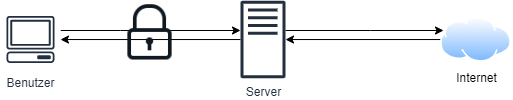
\includegraphics[width=0.8\textwidth]{VPN.png}
    \caption[Virtuelles privates Netzwerk]{Virtuelles privates Netzwerk} 
\end{figure} 

\newpage
\section{Interprozesskommunikation}
Interprozesskommunikation ist der Fachbegriff für die Kommunikation zwischen verschiedenen Prozessen auf demselben Rechner. Es gibt verschiedene Arten der Interprozesskommunikation, zum einen speicherbasierte Kommunikation in Form von Shared Memory oder Dateinen und zum anderen nachrichtenbasierte Kommunikation über Message Queues, Pipes oder Sockets.\footnote[1]{\cite[Vgl.][]{30}} 


\subsection{Shared Memory}
Mehrere Prozesse greifen auf gemeinsam genutzten Speicher lesend oder schreibend zu. Der Speicher wird von einem Prozess angefordert und dann mithilfe des Betriebssystems auch in den Adressraum der anderen Prozesse eingefügt, sodass jeder Prozess darauf zugreifen kann. Shared Memory ist eine sehr simple Form der Interprozesskommunikation, die einzige Schwierigkeit ist die Synchronisation der Prozesse, also das kein Prozess gleichzeitig mit einem anderen Prozess auf den gemeinsam genutzten Speicher zugreifen kann und es somit zu keinen Race Conditions kommt.$^{1}$


\subsection{Dateien}
Mehrere Prozesse greifen auf eine Datei zu, in diese Datei werden Daten von den Prozessen geschrieben beziehungsweise gelesen. Die Prozesse dürfen wie auch auf den Shared Memory nur synchronisiert zugreifen, oftmals erfolgt dies mithilfe des Betriebssystems das den Zugriff entweder auf nur einzelne Daten der Datei oder auf die ganze Datei sperrt.$^{1}$

\subsection{Message Queue}
Daten werden an eine Nachrichtenwarteschlange gesendet, diese hat eine eindeutige Kennung, sodass die anderen Prozesse wissen aus welcher Warteschlange sie die Daten beziehen müssen. Message Queues arbeiten entweder nach dem FIFO-Prinzip (First in First out) also die Daten, die als Erstes in die Warteschlange kommen, gehen auch als Erstes wieder raus oder mithilfe von Prioritäten, sodass Prozesse die Daten mit der höchsten Priorität als Erstes aus der Warteschlange nehmen.$^{1}$ 

\subsection{Pipes}
Die Pipe ist die erste Technik der Interprozesskommunikation, sie wurde für Unix entwickelt. Pipes kann man immer nur in eine Richtung verwenden, also ein Prozess schreibt immer und einer liest immer.  Um also Daten von einem Prozess zum anderen und wieder zurückzubefördern werden zwei unterschiedliche Pipes benötigt. Pipes sind wie auch die Massage Queues nach dem FIFO Prinzip aufgebaut. Es gibt zwei verschiedene Arten von Pipes die normalen/namenlosen Pipes und die benannten/FIFO Pipes. Der wesentliche Unterschied ist das namenlose Pipes nur von verwandten Prozessen verwendet werden können. Hingegen zu benannten Pipes die von jedem Prozess verwendet werden können, der den Namen der Pipe und die benötigten Berechtigungen hat, um eine Verbindung mit der Pipe aufzubauen.$^{1}$

\subsection{Sockets}
Zur Kommunikation mithilfe von Sockets wird ein Server und mindestens ein Client benötigt. Der Server hat  zu jedem Client ein Socket worüber er mit diesem kommunizieren kann. Die Kommunikation erfolgt in beide Richtungen. Der Plan für Sockets war das damit verschiedene Rechner über das Netzwerk miteinander kommunizieren können. Es ist aber auch möglich damit Interprozesskommunikation zu betreiben. Indem der Server und der Client beide am selben Rechner laufen.\footnote[1]{\cite[Vgl.][]{30}}